\ifx\wholebook\relax\else
\input{../Common.tex}
\input{../macroes.tex}
\begin{document}
\fi
\chapter{Methods: Named Message Sequences}\label{ch:turtleTeaching}\label{ch:abstraction}\label{cha:enseigner}

%\begin{chapterfigure}
%
\includegraphics[width=0.9\linewidth]{carosName}
%\end{chapterfigure}

%\begin{figure}
%\center{\includegraphics{microBrowserInWorking}}
%\caption{ .\label{fig:microBrowserInWorking}}
%\end{figure}


Up to now, you used scripts: you created \newcommand{\remove}[1]{first} a robot and sent a sequence of 
messages to it. Using scripts is a straightforward approach, but it has some 
severe limitations. One of the major \newcommand{\replace}[2]{limitation}{limitations} is that a script cannot be called by another script. This is a real problem because a script cannot be reused by other scripts. \newcommand{\replace}[2]{Moreover}{For instance,} you cannot decompose a complex problem into simpler problems \newcommand{\add}[1]{that you solve with separate scripts,} and then \newcommand{\replace}[2]{recompose}{combine} them to solve the complex problem.

Wouldn't it be nice if one could define a kind of script whose sequence of messages could be sent to any robot\newcommand{\replace}[2]{.}{?} Well, this is \newcommand{\replace}[2]{of course}{actually} possible\newcommand{\add}[1]{,} and such a sequence of messages is called a \emph{method}\footnote{In the context of this book we will not \newcommand{\replace}[2]{elaborate on}{go into} the \newcommand{\replace}[2]{real}{full} power of methods\newcommand{\add}[1]{,} as \newcommand{\replace}[2]{this has to do with}{it involves} 
object-oriented programming.}. A \emph{method} is a named sequence of messages. This name can be used in a script or even in another method.  In fact, all \newcommand{\add}[1]{the} robot messages \newcommand{\add}[1]{you have} used so far are methods that you \newcommand{\replace}[2]{used on}{can use with} any robot. 

In this chapter, you shall learn how to define methods. You already know most of \newcommand{\replace}[2]{the things needed}{what you need} to write the code of the methods. However \newcommand{\add}[1]{a} method must be defined using  a special editor called \index{code browser} \index{browser} a code browser. We start by comparing a script and a method. Then we will define a method\newcommand{\replace}[2]{ then}{, and} finally step back and really look in detail at what we did.


\section{Scripts versus Methods}
\newcommand{\replace}[2]{Let us}{Let's} look at one of the scripts you have \newcommand{\replace}[2]{been}{already} written\newcommand{\remove}[1]{ so far}, for
example\newcommand{\remove}[1]{, the} script~\ref{src:againSquare} that created a
robot and asked it to draw a \newcommand{\add}[1]{square} 100 pixels \newcommand{\replace}[2]{width square}{wide}. 
\begin{scriptwithtitle}{A simple square}\label{src:againSquare}
| \caro |
\caro := \Turtle new.
4 timesRepeat: 
   [ \caro turnLeft: 90.
   \caro go: 100 ]
\end{scriptwithtitle}
The problem with \newcommand{\replace}[2]{a}{this} script is that each time you need to draw a square
you need to \emph{copy} the 3 last lines of \scriptref{src:againSquare}.  \newcommand{\replace}[2]{In addition,}{Also} if you want \newcommand{\replace}[2]{that}{another robot (for example \daly) to draw} the square\newcommand{\remove}[1]{ be drawn by another robot, \daly for example}, you must change \newcommand{\remove}[1]{everywhere} the name \caro to \daly\newcommand{\add}[1]{ everywhere}. This is illustrated by \scriptref{src:againSquare2}.
\begin{scriptwithtitle}{Two simple squares}\label{src:againSquare2}
| \caro \daly |
\caro := \Turtle new.
\daly := \Turtle new.
\daly jump: 200.
\daly color: Color red.
\textbf{
4 timesRepeat: 
         [ \caro turnLeft: 90.
         \caro go: 100 ].
4 timesRepeat: 
         [ \daly turnLeft: 90.
         \daly go: 100 ].}
\end{scriptwithtitle}
\newcommand{\replace}[2]{Because of all this}{For all these reasons}, working with scripts is not easy. In
fact, we are quite convinced that the \newcommand{\replace}[2]{two following}{following two} statements
reflect \newcommand{\replace}[2]{you}{your} personal experience with scripts.
\begin{itemize}
\item Writing long scripts is a painful task.
\item Repeating long scripts is boring and error prone. 
\item When copying complex scripts, the likelihood of making a
programming\footnote{As opposed to a syntax error, which would be
caught quickly by the computer. \emph{Programming} errors, on the
contrary, are quite difficult to catch.}  error, such as omitting a
line, is high.
\end{itemize}

\newcommand{\replace}[2]{In fact}{Instead}, we would like to \emph{define \newcommand{\add}[1]{a sequence of messages} once and \newcommand{\replace}[2]{only once}{for all;}}\newcommand{\remove}[1]{ a sequence of messages,} to give \newcommand{\replace}[2]{it}{the sequence} a \emph{name}\newcommand{\add}[1]{;} and \newcommand{\add}[1]{then} to be able to \emph{send it as \newcommand{\add}[1]{a single} message to any\newcommand{\add}[1]{ robot}} \newcommand{\replace}[2]{robots}{---} just \newcommand{\replace}[2]{as any}{like the} predefined robot messages such as \go, \north, \jump... 
         
With \newcommand{\replace}[2]{such an}{this} approach we \newcommand{\add}[1]{could} define a new \emph{method} \ct{square}, and 
\newcommand{\replace}[2]{we can}{then} write \newcommand{\remove}[1]{the} \scriptref{src:againSquareMethod} --- \newcommand{\replace}[2]{Do not yet}{but don't} execute it 
\newcommand{\replace}[2]{since}{yet, because} the method \ct{square} has not yet been defined. \newcommand{\replace}[2]{What you see is}{But you can see} that we 
do not have to duplicate and adapt the sequence of messages defining a square\newcommand{\add}[1]{ anymore}. We \newcommand{\add}[1]{can} just use it twice. \newcommand{\replace}[2]{Now you should be}{\paragraph

We hope you are now} convinced that defining \newcommand{\add}[1]{the} method is worth the effort. 
   
\begin{scriptwithtitle}{Using the method \ct{square}}\label{src:againSquareMethod}
| \caro \daly | 
\caro := \Turtle new.  
\daly := \Turtle new.  
\daly go: 200.  
\daly color: Color red.
\textbf{\caro square.
\daly square}
\end{scriptwithtitle}


%%%%%%%%%%%%%%%%%%%%%%%%%%%%%%%%%%%%%%%%%%%%%%%%%%%
\section{How \newcommand{\replace}[2]{to}{Do We} Define a Method?}
In this section we give a cookbook recipe \newcommand{\replace}[2]{on how to create}{for creating} a method. 
\newcommand{\replace}[2]{As}{Since} in \newcommand{\remove}[1]{the context of} this book you will only define methods for \newcommand{\remove}[1]{the} robots, we programmed some \newcommand{\replace}[2]{simple and dedicated}{specialized} code browsers (\ie tools to define methods) \newcommand{\replace}[2]{that will let you define}{just for defining} methods for your robots. \newcommand{\replace}[2]{By default you get one}{There is a} \tb in the working flap, \newcommand{\replace}[2]{but}{or} you can always create one by \newcommand{\replace}[2]{grabbing}{dragging} its thumbnail from the dark blue flap. 
   
Using a \tb to define a method requires \newcommand{\add}[1]{you} to (1) choose or create a method
category \ie a kind of method folder (Section~\ref{sec:createCategory}), (2) type the method and (3) then compile it (Section~\ref{sec:definingmethod}). \newcommand{\replace}[2]{Let us}{\paragraph

Let's} detail the different parts of a \tb.
\subsection{\newcommand{\replace}[2]{A}{The} \tb}
\newcommand{\replace}[2]{As we already said, defining}{Defining} methods requires \newcommand{\remove}[1]{to use} a new \newcommand{\add}[1]{tool: the} editor shown in Figure~\ref{fig:methodEditor}. This browser is actually a simplified version of the browser used by \st programmers. 
\begin{figure}
@@dank: Suggestion for annotation at top of this graphic--
list of categories (\newcommand{\replace}[2]{folder}{folders} for methods)
Suggestions for annotations at bottom of graphic --
selected \newcommand{\replace}[2]{method}{method's} definition 
selected \newcommand{\replace}[2]{method}{method's} name and \newcommand{\replace}[2]{parameters}{parameter}
@@
\centerline{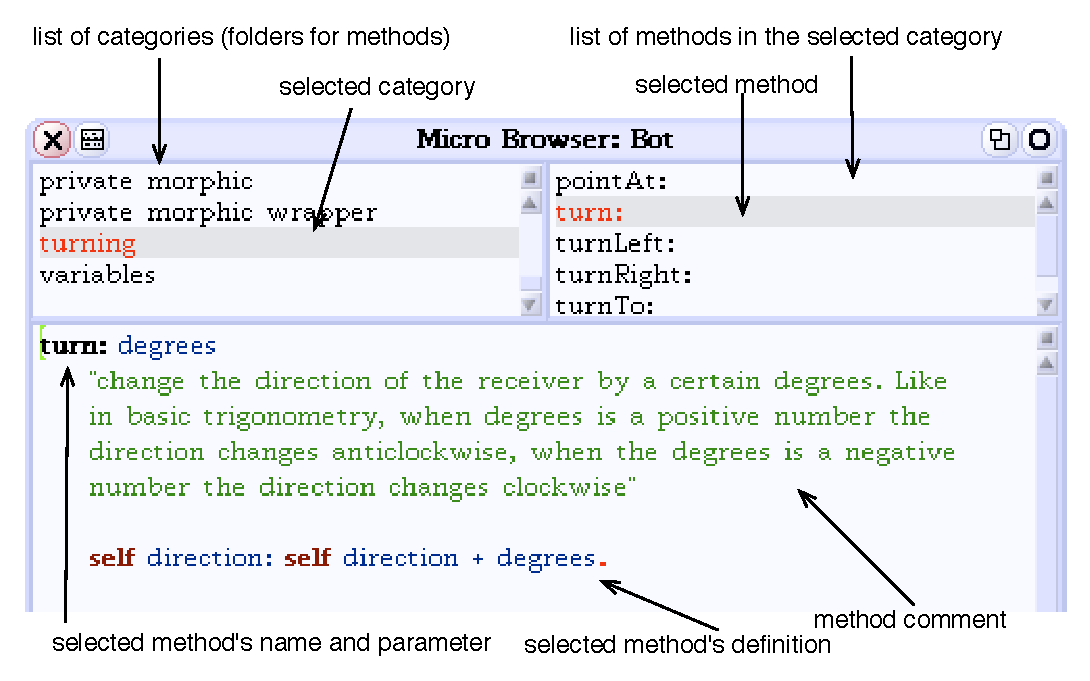
\includegraphics[width=10cm]{tbOneAnnotated}} 
\caption{The \tb showing the definition (\newcommand{\add}[1]{in the} bottom pane) of the 
method \ct{turn:} (\newcommand{\add}[1]{selected in the upper} right pane) belonging to the category \emph{turning} (\newcommand{\add}[1]{selected in the upper} left pane).\label{fig:methodEditor}}
\end{figure}
The browser consists of 3 parts\newcommand{\add}[1]{ or panes}:
\begin{description}
\item[Categories.] The \newcommand{\replace}[2]{left top}{upper left} part is the \emph{category list}.
It \newcommand{\replace}[2]{contains}{shows} the method categories. Method categories are just names
that \newcommand{\remove}[1]{help us to} group methods together so that we can find information
faster. In Figure~\ref{fig:methodEditor}, the category 'turning'
\newcommand{\replace}[2]{grouping}{is selected; it groups} all the operations having to \newcommand{\replace}[2]{deal}{do} with robot direction changes\newcommand{\remove}[1]{ is selected}. Other categories \newcommand{\replace}[2]{grouping}{that group} other robot \newcommand{\replace}[2]{behavior}{methods} are \newcommand{\add}[1]{also} listed.
\item[Methods.] The \newcommand{\replace}[2]{right top}{upper right} part is the \emph{method list}.
It \newcommand{\replace}[2]{contains}{shows} the method names of the methods \newcommand{\remove}[1]{contained} in the selected category. In Figure~\ref{fig:methodEditor}, five  methods are listed: \ct{pointAt:}, \ct{turn:}\newcommand{\replace}[2]{ and}{,} \turnLeft, \turnRight, and \ct{turnTo:}. The method named \ct{turn:} is currently selected.
\item[Method Definition.] The bottom part is the \emph{code \newcommand{\add}[1]{display and code} editor}. It shows the definition of the method whose name is selected. This is also \newcommand{\remove}[1]{the place} where you can type the code of a new method.
\end{description}

\subsection{Creating a New Method Category}\label{sec:createCategory} 
Methods are grouped by categories. A category is simply defined by a name. To start defining a method, you \newcommand{\replace}[2]{must first}{either} define \newcommand{\replace}[2]{its}{a new} category \newcommand{\add}[1]{for it,} or select \newcommand{\replace}[2]{a}{an existing} category \newcommand{\replace}[2]{in which you want to define}{for} your method. \newcommand{\replace}[2]{Let us}{Let's} create a new category named \newcommand{\replace}[2]{regular shapes}{\ct{regular polygons}}.

\begin{figure}
\centerline{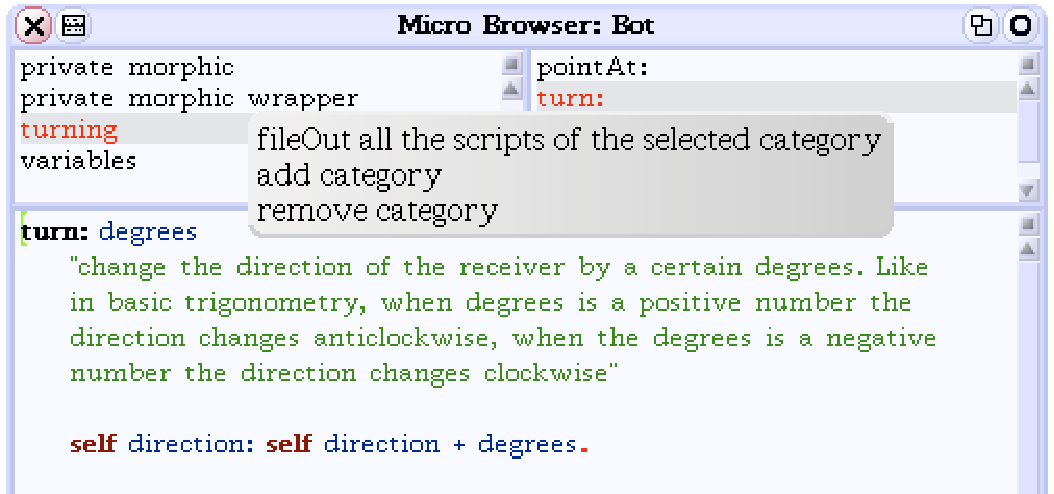
\includegraphics[width=10cm]{tbTwo}} 
\caption{To create a method category, \newcommand{\replace}[2]{in}{open} the category menu\newcommand{\replace}[2]{,}{ and} select 'add category'.\label{fig:categoryMenu}}
\end{figure}
\begin{figure}\label{fig:categoryPrompt}
\centerline{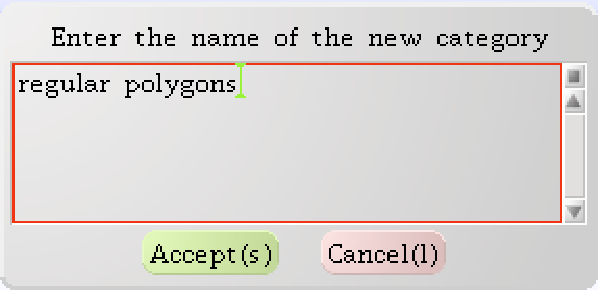
\includegraphics[width=6cm]{tbThree}}
 \caption{Entering the new category name.}
\end{figure}
\begin{enumerate}
\item Click with the right mouse button on the category list.
A menu \newcommand{\replace}[2]{such as}{like} the one \newcommand{\replace}[2]{of}{in} Figure~\ref{fig:categoryMenu} will show up.
\item Select the option \ct{add category} of that menu.
\item Type the name of the category in the dialog that pops up 
as shown in Figure~\ref{fig:categoryPrompt}.You may choose any name for the category. Of course, meaningful names are better \newcommand{\replace}[2]{if}{when} you want to share your work with other people\newcommand{\add}[1]{,} or find
your \newcommand{\replace}[2]{way quickly}{method again}. 
\item Click \newcommand{\remove}[1]{into} the \ct{Accept} button to validate your  choice.
\end{enumerate}


As shown in Figure~\ref{fig:categorycreated}\newcommand{\add}[1]{,} the name of the
new category appears in the category pane and is automatically
selected. The editor is ready to accept the new method definition. It shows 
you a reminder \newcommand{\replace}[2]{for the definition of}{of how to define a} method\newcommand{\replace}[2]{ that}{, which} you can remove when you start 
typing your method. \newcommand{\add}[1]{\paragraph
''
You are now ready to define your first method.
\begin{figure}
\centerline{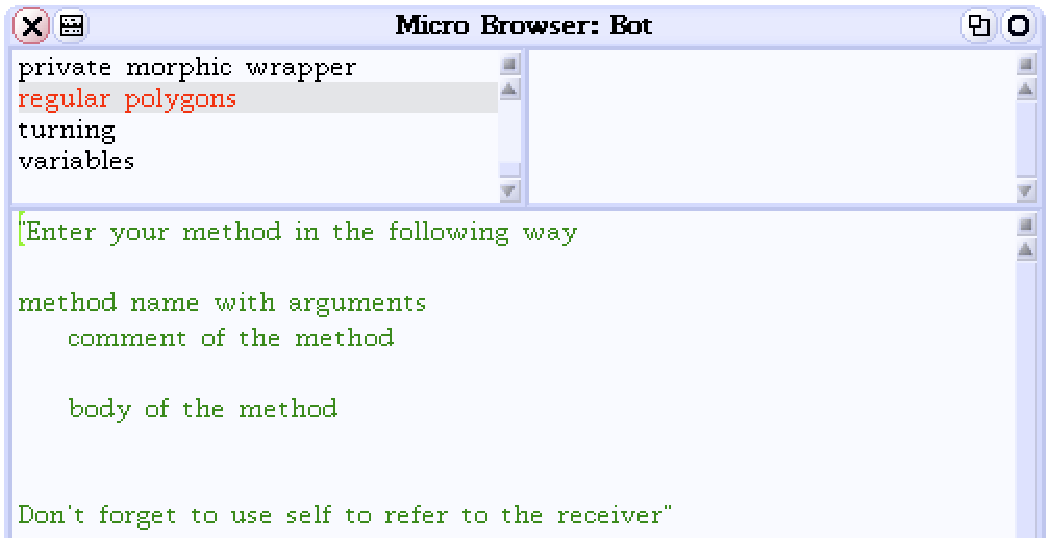
\includegraphics[width=10cm]{tbFour}}
\caption{The \newcommand{\replace}[2]{resulting}{new} category is \newcommand{\replace}[2]{created}{ready}.\label{fig:categorycreated}}
\end{figure}
\subsection{Defining your First Method}\label{sec:definingmethod}
If the category \newcommand{\replace}[2]{in}{to} which you want to add your method is not selected,
select it. Then type \newcommand{\replace}[2]{in the method as shown by}{the contents of} \methodref{mth:square}
\newcommand{\add}[1]{(}shown below\newcommand{\add}[1]{)} into the code editor pane. \newcommand{\replace}[2]{For that you can simply}{To do that,} select \newcommand{\replace}[2]{the 
previous text}{all the text in the code editor} and start typing your method. 
\begin{method}\label{mth:square}
square 
   "Draw a square \newcommand{\replace}[2]{of 100 pixel size}{100 pixels wide}"
   4 timesRepeat: 
                [ self go: 100.
                self turnLeft: 90 ]
\end{method}

Defining a method is a three step process:

\paragraph{1. Typing the method.} Typing code into the code editor 
pane works exactly as with the script editor. \newcommand{\replace}[2]{Just}{First} delete the \newcommand{\replace}[2]{text, which}{reminder text that} is in the code editor pane. To make this \newcommand{\replace}[2]{fast}{quick,} just \newcommand{\replace}[2]{position the cursor}{point your mouse} at 
the beginning of the editor \newcommand{\add}[1]{pane} before the first character and click. This will select \newcommand{\replace}[2]{the complete}{all of the} code editor text. \newcommand{\add}[1]{\paragraph
''
Once you \newcommand{\replace}[2]{typed}{finish typing} the \newcommand{\add}[1]{new} method\newcommand{\add}[1]{,} your screen should \newcommand{\remove}[1]{then} look like \newcommand{\remove}[1]{the one of} Figure~\ref{fig:firstMethod}.
\begin{figure}
\centerline{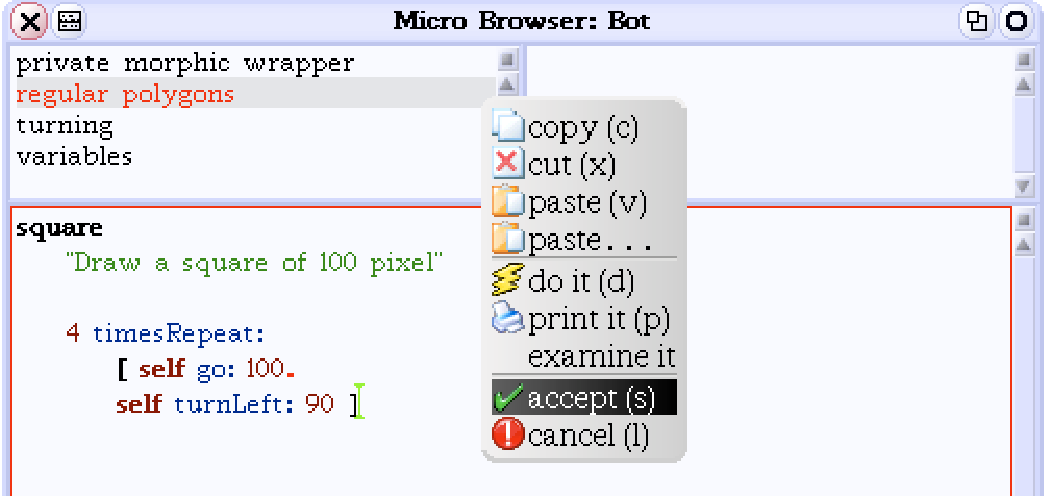
\includegraphics[width=10cm]{tbFive}} 
\caption{You have typed \newcommand{\add}[1]{in} the method \ct{square}\newcommand{\replace}[2]{ and now}{. Now} you should compile it using the code editor menu.\label{fig:firstMethod}}
\end{figure}
\paragraph{2. Compiling the method.} As shown by Figure~\ref{fig:compileMethod}, click to bring \newcommand{\add}[1]{up} the menu  \newcommand{\replace}[2]{of}{for} the code editor and select the option \menu{Accept}.
This compiles the method \ie \newcommand{\replace}[2]{transform}{transforms} its definition into a representation that \newcommand{\replace}[2]{a}{the} computer can understand and execute. A new method named \ct{square} appears in the method list.  \newcommand{\replace}[2]{Note that if}{If} you made \newcommand{\add}[1]{a} mistake while typing the method, \sq will report \newcommand{\replace}[2]{errors as we already discussed}{the error as it would for a script}.

If you define \newcommand{\remove}[1]{correctly} the method\newcommand{\add}[1]{ correctly}, you should be able to compile it\newcommand{\replace}[2]{, the}{without \sq reporting any errors. The} browser \newcommand{\replace}[2]{reflects}{will then reflect} the fact that the compilation is done and that robots can now understand messages with the new method\newcommand{\add}[1]{,} by showing the \newcommand{\replace}[2]{method}{new method's} name in the method \newcommand{\remove}[1]{category} list (see Figure~\ref{fig:methodskeleton}).

%	\begin{figure}
%	\centerline{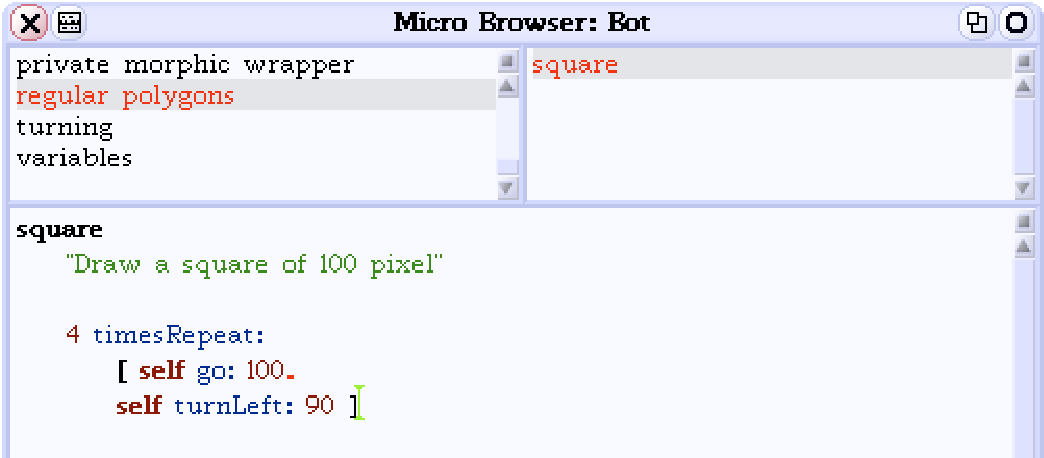
\includegraphics[width=15cm]{tbSix}} 
%	\caption{You have typed \newcommand{\remove}[1]{the method} and \newcommand{\replace}[2]{compile}{compiled} the method \ct{square} 
%	\newcommand{\replace}[2]{now the}{. The} browser reflects the fact that \newcommand{\replace}[2]{robot}{robots} can understand messages with the 
%	new method.\label{fig:compileMethod}}
%	\end{figure}
\paragraph{3. Testing the method!} You \newcommand{\remove}[1]{do not} have \newcommand{\add}[1]{not} finished yet\newcommand{\add}[1]{,} because 
the method you \newcommand{\replace}[2]{type}{defined} \newcommand{\replace}[2]{may}{could} be wrong\newcommand{\replace}[2]{ so you}{. You} should test it.  Execute the
\scriptref{src:againSquareMethod}\newcommand{\add}[1]{ by sending a message with the new method's name \ct{square} to a robot}.

\newcommand{\replace}[2]{At this point you should realize}{Notice} that a method can be reused several times\newcommand{\add}[1]{,} as demonstrated by \scriptref{src:againSquareMethod}.  \newcommand{\replace}[2]{Note that this fact this}{This} is \newcommand{\replace}[2]{not new}{old news}. 
You \newcommand{\add}[1]{have} used \newcommand{\replace}[2]{that}{this fact} since the beginning of this book: messages such as \go, \turnLeft and so on, are \newcommand{\replace}[2]{implemented as methods, just like}{methods defined in the same way as} the method \ct{square}. 

%%%%%%%%%%%%%%%%%%%%%%%%%%%%%%%%%%%%%%%%%%%%%%%%%%%
\section{What's in a Method?}
We asked you to type a method without much explanation. Now is the time to
analyze the structure of the method. \newcommand{\add}[1]{\paragraph
''
A method is composed of a \emph{name}, an optional \emph{method comment} and a \emph{method body} (a sequence of messages) as shown by Figure~\ref{fig:methodskeleton}. \newcommand{\replace}[2]{To be exact, the}{The} method name can also contain parameters (\newcommand{\replace}[2]{See}{see}
chapter~\ref{ch:argumenting}), and the method body can \newcommand{\remove}[1]{contain} also
\newcommand{\replace}[2]{definition of}{define} local variables using vertical bars \ct{|} and \ct{|}.
\begin{figure}
\centerline{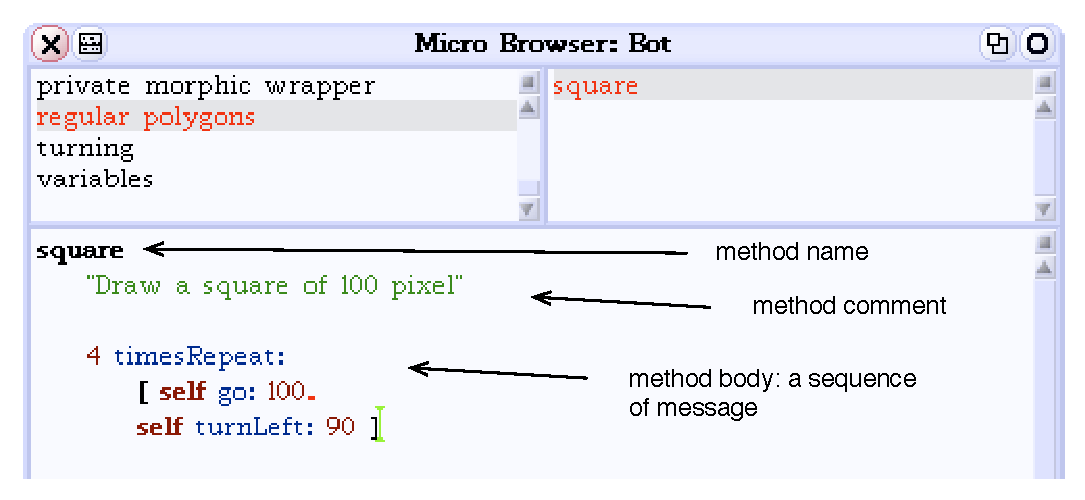
\includegraphics[width=15cm]{tbSixAnnotated}} 
\caption{A method is composed of a name, a method comment and a 
method body. \label{fig:methodskeleton}}
\end{figure}

\largecadre{A method name should always represent what the method does\newcommand{\replace}[2]{ 
and}{,} not how it does it.}

\begin{description}
\item[Method Name.] 
A method name should always represent what the method does\newcommand{\replace}[2]{ 
and}{,} not how it does it.  When you want \newcommand{\remove}[1]{to} somebody to open a door, 
you \newcommand{\replace}[2]{do not}{don't} explain \newcommand{\remove}[1]{him} all the \newcommand{\replace}[2]{physic}{physics} and mathematics involved. \newcommand{\replace}[2]{This}{It} is the 
same for \newcommand{\replace}[2]{method}{methods}. 

Method names without parameters such as 
\ct{square} follow the same syntax as variable names. They are 
composed of \newcommand{\replace}[2]{alphanumerical}{alphanumeric} characters \newcommand{\add}[1]{(letters and digits),} and start with a
lowercase character. In our case the method name is \ct{square}.
\item[Method Comment.]
\newcommand{\replace}[2]{It}{A comment} consists of \newcommand{\remove}[1]{a} text enclosed \newcommand{\replace}[2]{within a pair of}{between} double quotes
(\ct{"}). \newcommand{\replace}[2]{That}{The} text cannot contain any double quotes. However\newcommand{\remove}[1]{,} a
comment can be as long as you like\newcommand{\add}[1]{,} and can \newcommand{\replace}[2]{span itself}{continue}
over several lines. \newcommand{\add}[1]{\paragraph
''
In general a comment explains the purpose and the 
effect of the method. It explains how the method can be used\newcommand{\replace}[2]{ and}{,} not how 
the method \newcommand{\replace}[2]{is working}{does its job}. \newcommand{\replace}[2]{People}{Anyone} who wants to know how the method \newcommand{\replace}[2]{is defined should}{works can} read the method's body.

If the method name is \newcommand{\replace}[2]{explicit}{clear} enough, the comment may be omitted.  
In our case the method comment is:
\begin{nalltt}
   "Draw a square \newcommand{\replace}[2]{of 100 pixel size}{100 pixels wide}"
\end{nalltt}

\item[Method Body.] After the comment comes the method definition itself
\ie the sequence of messages that are executed in response to a message. In our case the 
method body is: 
\


\begin{nalltt}
   4 timesRepeat: 
         [ self go: 100.
         self turnLeft: 90 ]
\end{nalltt}
\end{description}
       
\largecadre{A method is a named sequence of messages. It is composed of
a name, a comment and a sequence of messages. Once a method is defined\newcommand{\add}[1]{,} any robot can execute it in \newcommand{\replace}[2]{answer}{response} to a message with the same name.}       
\subsection{Script vs. Method: an Analysis}
If you compare \newcommand{\remove}[1]{the} \methodref{mth:square} with \newcommand{\remove}[1]{the} \scriptref{src:againSquare}\newcommand{\add}[1]{,} you \newcommand{\replace}[2]{notice following}{can see these} differences:
\begin{itemize}
\item The line declaring the variable \caro is \newcommand{\replace}[2]{no longer here}{not in the method}.
\item The line creating the robot \newcommand{\replace}[2]{has been suppressed}{is not there, either}.
\item In \newcommand{\replace}[2]{all other lines}{the rest of the method}, the variable \caro is replaced by \self.
\end{itemize}
\newcommand{\replace}[2]{This should not be a surprise, since we already announced}{Remember} that a
\newcommand{\add}[1]{\Bot} method represents a sequence of messages which can be sent to
\emph{any} robot: the robot \newcommand{\replace}[2]{refered}{referred to} by the variable \caro is not necessarily the
receiver of the message \ct{square}. As we saw \newcommand{\replace}[2]{before}{in \scriptref{src:againSquare2},} \daly \newcommand{\replace}[2]{can}{could} also be \newcommand{\replace}[2]{a message}{the} receiver
of the message \ct{square}. \newcommand{\replace}[2]{Then}{\paragraph

Also}, the message \ct{square} is sent to an \emph{existing}
robot. \newcommand{\replace}[2]{Thus, there}{There} is no need to create a robot since the one we want to send message to already
exists. \newcommand{\replace}[2]{This implies that}{So} while defining the method \ct{square}, we \newcommand{\replace}[2]{must have}{need} a way to refer to the object that will receive the message \ct{square}.  \newcommand{\replace}[2]{Indeed}{In fact}, we want to send \newcommand{\add}[1]{the sequence of
messages specified within the method body} to the \newcommand{\add}[1]{specific} object
receiving the message \ct{square} and \newcommand{\replace}[2]{only to this one, the sequence of
messages specified in the method body}{to no other}. Therefore we need a way to refer to the receiver of a message.  This is the purpose of \self. Inside a method, \self represents the object receiving \newcommand{\replace}[2]{a}{the}  message.

\paragraph{The \self variable.}
If you remember the discussion of Chapter~\ref{ch:variables}, a
variable is just a named placeholder for an object. In particular, we emphasized 
that the same variable could be used to point to different objects\newcommand{\replace}[2]{.}{ at different times.\paragraph
} 
In the case of a method, the variable \self points to the object that \newcommand{\replace}[2]{receives}{received} the message: when the message \ct{\caro\ square} is executed \self refers to the robot named \caro, \newcommand{\add}[1]{and} when the
message \ct{\daly\ square} is executed \self refers to the robot named \daly.
\newcommand{\replace}[2]{To be complete,}{\paragraph
}
\self is a special variable because you cannot change its value. Only \sq can assign the value of \self. That's why \self does not have to be declared between vertical bars \ct{|}. Moreover, \self can only the used inside a method definition.
\largecadre{Inside a method the variable \ct{self} represents the 
object that \newcommand{\replace}[2]{receives}{received} the message. \newcommand{\replace}[2]{Therefore if messages have to be sent}{When the method code needs to send a message} to the receiver, send \newcommand{\replace}[2]{messages}{the message} to \self\newcommand{\add}[1]{.}}

\paragraph{Method or Not: That's the Question.} At this stage you may be tempted to go back and convert all \newcommand{\add}[1]{the} scripts you have \newcommand{\replace}[2]{been doing}{written} into methods. This is not advisable\newcommand{\replace}[2]{ since}{, because} not all scripts are worth \newcommand{\replace}[2]{themselves to be turned}{turning} into a method. In general, one \newcommand{\replace}[2]{makes}{should define} a method when \newcommand{\replace}[2]{a}{the} sequence of messages is \newcommand{\remove}[1]{sufficiently} general \newcommand{\add}[1]{enough} to be used several times.

\section{Returning a Value}
A method can also return a value \newcommand{\add}[1]{by} using the character up arrow \^\\newcommand{\add}[1]{,} also called  \index{return} \index{caret} \index{returning a value} \newcommand{\replace}[2]{caret.}{a \emph{caret}.\paragraph
}
Imagine that we want to have a method that returns the \newcommand{\replace}[2]{length}{distance} that a robot should move in one movement. We can define the method \ct{\newcommand{\replace}[2]{maxLength}{moveDistance}} shown in~\ref{mth:maxLength}. \newcommand{\replace}[2]{Here}{In this example} the method is simply returning a number\newcommand{\add}[1]{,} but we \newcommand{\replace}[2]{can}{could instead} return the result of \newcommand{\replace}[2]{any}{some} complex expression. 

\begin{method}\label{mth:maxLength}
\newcommand{\replace}[2]{maxLength}{moveDistance} 
   "returns the \newcommand{\replace}[2]{maximum length\newcommand{\add}[1]{distance to move}"

   ^ 100
\end{method}

By default every method returns the message receiver. The method~\ref{mth:squareEquivalent} is equivalent to the method \ct{square} defined previously. In fact at the end of every method there is an implicit expression \^ \self. However in \newcommand{\remove}[1]{the context of} this book you do not have to worry about that. 

\begin{method}\label{mth:squareEquivalent}
squareEquivalent
   "Draw a square \newcommand{\replace}[2]{of 100 pixel size}{100 pixels wide}"
   4 timesRepeat: 
              [ self go: 100.
              self turnLeft: 90].
   ^ self
\end{method}

In the context of this book we will not use \newcommand{\remove}[1]{a lot} this feature \newcommand{\add}[1]{much,} but \newcommand{\replace}[2]{this}{it} is important to know that a method always returns a value. 

\section{Pattern Drawing}\label{sec:newart}
Now it is time to practice. As you have seen, it is quite easy to transform a script into a method.  Many seasoned programmers use scripts to test ideas. When the feasibility of an idea has been proven in the form of a script, they move the code of the script into a method for later reuse. The next exercise trains you to do exactly this.
\newcommand{\replace}[2]{Let us}{Let's} consider the following script~\ref{src:artNouveau} which draws a geometric shape. 
\begin{scriptfig}{artNouveauScr}{A Simple Pattern}\label{src:artNouveau}
| \caro |
\caro := \Turtle new.
\caro go: 100 ;
        turnLeft: 90 ;
        go: 100 ;
        turnLeft: 90 ;
        go: 50 ;
        turnLeft: 90 ;
        go: 50 ;
        turnLeft: 90 ;
        go: 100 ;
        turnLeft: 90 ;
        go: 25 ;
        turnLeft: 90 ;
        go: 25 ;
        turnLeft: 90 ;
        go: 50
\end{scriptfig}
\begin{exonofig} \label{exo:artNouveau}
Create a method named \ct{pattern} which produces the \newcommand{\replace}[2]{drawing presented in Figure}{figure drawn by} \scriptref{src:artNouveau}.
\end{exonofig}
We now can use this method in a script to draw a frame.
\begin{scriptfig}{artNouveauFourScr}{A Frame} 
\label{src:artNouveauFrame}
| \caro |
\caro := \Turtle new.
4 timesRepeat: [ \caro pattern ; go: 50 ]
\end{scriptfig}
At this point, some astute reader might ask: why don't we create a
method---named \ct{frame50}, for example---corresponding to
that of \scriptref{src:artNouveauFrame}\newcommand{\replace}[2]{}{?}. This is indeed possible
since \emph{any method created for \newcommand{\add}[1]{a} robot can be reused
by another \newcommand{\replace}[2]{turtle}{robot} method}. This is the topic of the next chapter. 
\begin{exonofig} \label{exo:artNouveauFrame50}
Create a method named \ct{frame50} which produces the picture produced by Script \ref{src:artNouveauFrame}. 
\end{exonofig}

\comment{
\newcommand{\replace}[2]{Nevertheless, let us}{Let's} convert one script, namely \scriptref{src:petal}
\newcommand{\replace}[2]{drawing}{that draws} a petal.
\begin{exonofig} \label{exo:mthPetal45}
Write a method named \ct{petal} corresponding to 
\scriptref{src:petal}. 
\end{exonofig}

In order to test whether the new method you created is correct,
you must write a simple script to test it, a script similar to
Script \ref{src:petal}. After \newcommand{\replace}[2]{this}{that}, try \newcommand{\replace}[2]{to use}{using} the method in a
more complex script.
\begin{exonofig} \label{exo:usePetal45}
Rewrite the script you \newcommand{\remove}[1]{have} made for Exercise \ref{exo:flower} to
use the new method \ct{petal45}.
\end{exonofig}
}

\summa

\begin{enumerate}
\item A method is a named sequence of messages. It is composed of
a name, a comment and a sequence of messages. Once a method is defined\newcommand{\add}[1]{,} any robot can execute it in \newcommand{\replace}[2]{answer}{response} to a message with the same name.

\item A method name should always represent what the method does\newcommand{\replace}[2]{ 
and}{,} not how it does it. 

\item A new method for a robot is created using a \tb \ie a special 
editor \newcommand{\replace}[2]{to define}{for defining} methods. 
\item Inside a method the variable \ct{self} represents the 
object that \newcommand{\replace}[2]{receives}{received} the message. \newcommand{\replace}[2]{Therefore if messages have to be sent}{When the method code needs to send a message} to the receiver, send \newcommand{\replace}[2]{messages}{the message} to \self\newcommand{\add}[1]{.}
\end{enumerate}


\subsection*{Glossary}
\begin{itemize}
\item Method categories. A method category is \newcommand{\add}[1]{a} folder in which methods are sorted. It helps \newcommand{\replace}[2]{finding}{you find} methods faster. 
\item Method. A method represents a sequence of messages that an object can execute. A method has a name. It is executed when an object receives a message having the same name. 
\item Browser. A browser is a special tool \newcommand{\replace}[2]{to view and edit}{for viewing and editing} methods. 
\item Comment. A comment is a piece of text \newcommand{\replace}[2]{delimited}{surrounded} by "" that \newcommand{\replace}[2]{indicates}{explains} the purpose of a method. 
\item \self. \self is a variable \newcommand{\remove}[1]{known} predefined \newcommand{\replace}[2]{in}{by} \st that always represents the receiver of the message. 
\end{itemize}

\ifx\wholebook\relax\else\end{document}\fi
